\documentclass[11pt,a4paper]{article}
\usepackage[T1]{fontenc}
\usepackage[utf8]{inputenc}
\usepackage[polish]{babel}
\usepackage{amsmath}
\usepackage{amsfonts}
\usepackage{graphicx}
\author{Kamil Kuczaj}
\title{Sprawozdanie z Laboratorium 3 - Pomiar czasu znajdywania losowego słowa z listy.\\Implementacja listy, stosu oraz kolejki przy wykorzystaniu odpowiednich interfejsów.}
\date{\today}
\begin{document}

\maketitle

\section{Wstęp}
Podanym zadaniem był pomiar czasu znajdywania losowego elementu listy typu\textit{string}. Należało wykonać pomiary zapisu: $10^1$, $10^3$ oraz $10^5$. Wykorzystano słownik $109582$ najpopularniejszych słów w języku angielskim. Zdecydowano się na wybór języka angielskiego nad polskim z uwagi na zlikwidowanie problemów z wczytywaniem znaków łacińskich. W programie zaimplementowano szablony, dzięki czemu bardzo łatwo jest zmierzyć czas dla innych zmiennych lub nawet własnych klas.

Słowa w słowniku posortowane są alfabetycznie, więc za każdym razem do struktury danych były wczytywane będąc już uprzednio posortowane rosnąco.

\section{Specyfikacja komputera}

\begin{center}
	\begin{tabular}{| r | c |}
	\hline
	Wersja kompilatora \textit{g++} & 4.8.4 \\ \hline
	System & Ubuntu 14.04.4 \\ \hline
	Procesor	 & Intel Core i5 2510M 2.3 GHz \\ \hline
	Pamięć RAM & 8 GB DDR3 1600 MHz \\ \hline
	Rozmiar zmiennej \textit{int} & 4 bajty \\ \hline
	\end{tabular}
\end{center}

\section{Pomiary oraz ich interpretacja}
\bigskip

Bardzo dużą część czasu zajmowało zapisanie stu tysięcy słów - wynikało to z tego, że należało zaalokować pamięć, w tym wypadku zwiększając ją o jeden element za każdym razem. Wiąże się to ze złożonością obliczeniową rzędu $n^2$ w notacji dużego $\Theta$.\\\\
W programie użyłem funkcji \textit{rand()} z biblioteki \textit{<cstdlib>} do wylosowania losowego slowa ze slownika $109582$ najpopularniejszych słów w języku angielskim. Następnie przeszukiwałem listę w poszukiwaniu tego słowa i zapisywałem go do pliku niezależnie od tego, czy słowo zostało znalezione. Chciałem w ten sposób pokazać, że przeszukanie listy jest bardzo efektywne. Poniżej w tabeli przedstawione zostały średnie wyniki pomiarów.\\\\\\

\begin{table}[h]
\begin{center}

\begin{tabular}{|l|c|c|c|}
	\hline
	\textbf{Ilość elementów} & $10^1$ & $10^3$ & $10^5$ \\ \hline
	\textbf{Średni czas [$\mu$s]} & 9871,2 & 9323,78 & 13611,46 \\ \hline
    \textbf{Średni czas [s]} & 0,0098712	& 0,00932378	 & 0,01361146 \\ \hline


\end{tabular}

\end{center}
\caption{Wyniki pomiarów. Łatwo zauważyć, że przeszukanie listy trwa bardzo krótko i prawie nie zależy od ilości elementów}
\end{table}

\bigskip
\bigskip
\bigskip

Wydawać by się mogło, że liczenie średniej z pomiarów, gdzie nie uwzględnia się czy słowo zostało znaleziono, lub gdzie się znajdowało może być niedokładne. Jednak wyraźnie widać, że to skomplikowanie pomiarów miało by nieznaczny wpływ na uzyskane wyniki.

\begin{figure}[h]

\begin{center}
	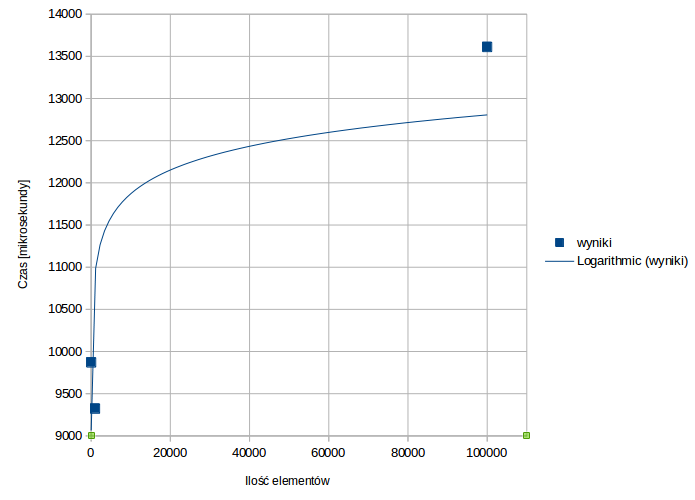
\includegraphics[scale=0.6]{../wyniki/wyniki_przeszukania.png}
\end{center}
\caption{Zobrazowanie wyników pomiaru oraz regresja logartymiczna wykonana w programie \textit{LibreOffice Calc}}
\end{figure}
\newpage
\section{Wnioski}
\hspace{4ex}Zastosowanie struktury danych typu \textit{lista} zdecydowanie pozwoliło zmniejszyć czas na znalezienie słowa. Dysponując podanymi danymi zakwalifikowałbym przeszukanie tablicy jako algorytm rzędu $log(n)$ w notacji dużego $\Theta$.
\end{document}